\titledquestion{Multiple Choices}

Each question has \textbf{one or more} correct answer(s). Select all the correct answer(s). For each question, you will get 0 points if you select one or more wrong answers, but you will get 1 point if you select a non-empty subset of the correct answers.

Write your answers in the following table.

%%%%%%%%%%%%%%%%%%%%%%%%%%%%%%%%%%%%%%%%%%%%%%%%%%%%%%%%%%%%%%%%%%%%%%%%%%%
% Note: The `LaTeX' way to answer a multiple-choices question is to replace `\choice'
% with `\CorrectChoice', as what you did in the previous questions. However, there are 
% still many students who would like to handwrite their homework. To make TA's work 
% easier, you have to fill your selected choices in the table below, no matter whether 
% you use LaTeX or not.
%%%%%%%%%%%%%%%%%%%%%%%%%%%%%%%%%%%%%%%%%%%%%%%%%%%%%%%%%%%%%%%%%%%%%%%%%%%

\begin{table}[htbp]
	\centering
	\begin{tabular}{|p{1.7cm}|p{1.7cm}|p{1.7cm}|p{1.7cm}|p{1.7cm}|p{1.7cm}|p{1.7cm}|p{1.7cm}|}
		\hline
		(a) & (b) & (c) & (d) & (e) & (f) \\
		\hline
		%%%%%%%%%%%%%%%%%%%%%%%%%%%%%%%%%%%%%%%%%%%%%%%%%%%%%%%%%%
		% YOUR ANSWER HERE.
		 B   &  CD   &  ABC   &  D   &  AB   &  C   \\
		%%%%%%%%%%%%%%%%%%%%%%%%%%%%%%%%%%%%%%%%%%%%%%%%%%%%%%%%%%
		\hline
	\end{tabular}
\end{table}

\begin{parts}
	\part[2] An undirected connected graph is a tree if and only if the graph
	\begin{choices}
		\choice is a simple graph.
		\CorrectChoice is cycle-free.
		\choice is a planar.
		\choice is bipartite.
	\end{choices}


	\part[2] If we use breadth first alogorithm to traverse the following graph, which are the possible order of visiting the nodes?

	\begin{center}
		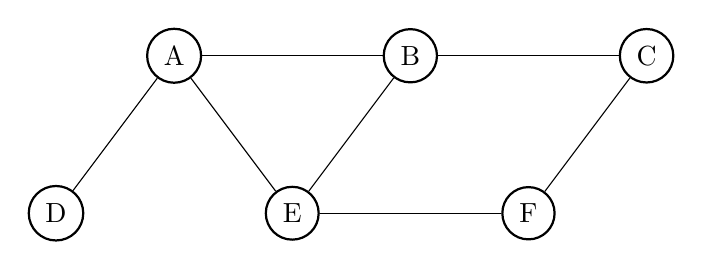
\begin{tikzpicture}
			\begin{scope}[every node/.style={circle,thick,draw}]
				\node (A) at (0,0) {A};
				\node (B) at (3,0) {B};
				\node (C) at (6,0) {C};
				\node (D) at (-1.5, -2) {D};
				\node (E) at (1.5, -2) {E};
				\node (F) at (4.5, -2) {F} ;
			\end{scope}
			\begin{scope}[ every node/.style={fill=white,circle}]
				\path [-] (A) edge (B);
				\path [-] (A) edge (D);
				\path [-] (A) edge (E);
				\path [-] (B) edge (C);
				\path [-] (B) edge (E);
				\path [-] (C) edge (F);
				\path [-] (E) edge (F);
			\end{scope}
		\end{tikzpicture}
	\end{center}
	\begin{choices}
		\choice DABCFE
		\choice BAECFD
		\CorrectChoice CBFAED
		\CorrectChoice ADEBFC
	\end{choices}

	\part[2] Which of the following statements are true for graph traversal?
	\begin{choices}
		\CorrectChoice Given two vertices in a graph \(s\) and \(t\), we can use both BFS and DFS to determine whether there exist a path from \(s\) to \(t\).
		\CorrectChoice Both DFS and BFS require \(\Omega(V)\) storage for their operation.
		\CorrectChoice Assuming we use queue to implement BFS. Let \(d(v)\) be the minimum number of edges between \(v\) and the start vertex. For any two vertices \(u, v\) in the queue, \(|d(u) - d(v)| \leq 2\).
		\choice A DFS of a directed graph always traverse through all the nodes.
	\end{choices}

	\part[2] Which of the following statements are true for graph traversal?

	\begin{choices}
		\choice A directed graph with \(n\) nodes and \(2n\) edges is strongly connected.
		\choice Graph with odd number of vertices cannot be a bipartite graph.
		\choice If a graph with \(n\) vertices has \(n - 1\) edges, it must be a tree.
		\CorrectChoice Undirected graph \(G = (V,E)\) is stored in an adjacency matrix A. The degree of \(V_i\) is \(\sum{j = 1}^{|V|}A[i][j]\).
	\end{choices}


	\part[2] Consider a tree generated by disjoint set union with union-by-rank (height) strategy of height $5$.
	Select the possible number nodes in the tree.
	\begin{choices}
		\CorrectChoice 114514
		\CorrectChoice 32
		\choice 5
		\choice 31
	\end{choices}
	\part[2] Which of the following statements concerning the complexity of union-find data structure strategies are correct?
	Union-by-rank: merge the tree with smaller height into a taller one.
	Union-by-size: merge the tree with smaller size (number of nodes) into a bigger one.
	\begin{choices}
		\choice When considering the asymptotic growth of the worst case running time, union-by-height is better than union-by-size.
		\choice For a tree with $n$ nodes generated by disjoint set union with union-by-rank, the height of the tree is $\Omega(\log n)$.
		\CorrectChoice For a tree with $n$ nodes generated by disjoint set union with union-by-size, the height of the tree is $O(\log n)$.
		\choice The worst-case running time complexity of a ``find'' operation in a disjoint set is so small that we can treat it as a constant.
	\end{choices}

\end{parts}
